\section{Michal Bros}
\label{sec:michalbros}

Wyrażenie matematyczne: $$\sum_{k=1}^{\infty}\frac{1}{k^2+1}$$

O to jest zdjecie Pandy~\ref{fig:pandzia}.

\begin{figure}[htbp]
    \centering
    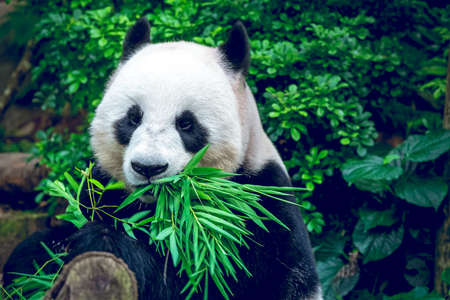
\includegraphics[width=0.2\textwidth]{pictures/pandzia.png}
    \caption{Ta Panda jest bardzo fajna.}
    \label{fig:pandzia}
\end{figure}

Tabela~\ref{tab:michalbros_tab} przedstawia macierz.
\begin{table}[htbp]
\begin{tabular}{|llll|}
1 & 0 & 0 & 0   \\
0 & 1 & 0 & 0   \\
0 & 0 & 1 & 0   \\
0 & 0 & 0 & 1  
\end{tabular}
\label{tab:michalbros_tab}
\caption{To jest moja macierz}
\end{table}

Co jedzą pandy ~\ref{itemize:mbros_list1}:
\begin{itemize}
  \item[>] jabłka.
  \item[>] żeń-szeń.
  \label{itemize:mbros_list1}
\end{itemize}

Gdzie są pandy ~\ref{itemize:mbros_list2}:
\begin{enumerate}
  \item W ZOO.
  \item W Azji.
  \label{itemize:mbros_list2}
\end{enumerate}

Fajne akapity ~\ref{akapit:mbros_akapit1}: 
\begin{center}
    Fajny \textbf{akapit} \par
    Fajny \underline{drugi akapit} 
    \label{akapit:mbros_akapit1}
\end{center}